%%%%%%%%%%%%%%%%%%%%%%%%%%%%%%%%%%%%%%%%%%%%%%%%%%%%%%%%%%%%%%%%%%%%%%%%%%%%%%%%%%%%%%
% Modelo de relatório de Disciplina de MLP a partir da
% classe latex iiufrgs disponivel em http://github.com/schnorr/iiufrgs
%%%%%%%%%%%%%%%%%%%%%%%%%%%%%%%%%%%%%%%%%%%%%%%%%%%%%%%%%%%%%%%%%%%%%%%%%%%%%%%%%%%%%%

%%%%%%%%%%%%%%%%%%%%%%%%%%%%%%%%%%%%%%%%%%%%%%%%%%%%%%%%%%%%%%%%%%%%%%%%%%%%%%%%%%%%%%
% Definição do tipo / classe de documento e estilo usado
%%%%%%%%%%%%%%%%%%%%%%%%%%%%%%%%%%%%%%%%%%%%%%%%%%%%%%%%%%%%%%%%%%%%%%%%%%%%%%%%%%%%%%
%
\documentclass[rel_mlp]{iiufrgs}

%%%%%%%%%%%%%%%%%%%%%%%%%%%%%%%%%%%%%%%%%%%%%%%%%%%%%%%%%%%%%%%%%%%%%%%%%%%%%%%%%%%%%%
% Importação de pacotes
%%%%%%%%%%%%%%%%%%%%%%%%%%%%%%%%%%%%%%%%%%%%%%%%%%%%%%%%%%%%%%%%%%%%%%%%%%%%%%%%%%%%%%
% (a A seguir podem ser importados os pacotes necessários para o documento, de acordo 
% com a necessidade)
%
\usepackage[brazilian]{babel}	    % para texto escrito em pt-br
\usepackage[utf8]{inputenc}         % pacote para acentuação
\usepackage{graphicx}         	    % pacote para importar figuras
\usepackage[T1]{fontenc}            % pacote para conj. de caracteres correto
\usepackage{times}                  % pacote para usar fonte Adobe Times
\usepackage{enumerate}              % para lista de itens com letras
\usepackage{breakcites}
\usepackage{titlesec}
\usepackage{enumitem}
\usepackage{titletoc}               
\usepackage{listings}			    % para listagens de código-fonte
\usepackage{mathptmx}               % p/ usar fonte Adobe Times nas formulas matematicas
\usepackage{url}                    % para formatar URLs
%\usepackage{color}				    % para imagens e outras coisas coloridas
%\usepackage{fixltx2e}              % para subscript
%\usepackage{amsmath}               % para \epsilon e matemática
%\usepackage{amsfonts}
%\usepackage{setspace}			    % para mudar espaçamento dos parágrafos
%\usepackage[table,xcdraw]{xcolor}  % para tabelas coloridas
%\usepackage{longtable}             % para tabelas compridas (mais de uma página)
%\usepackage{float}
%\usepackage{booktabs}
%\usepackage{tabularx}
%\usepackage[breaklinks]{hyperref}

\usepackage[alf,abnt-emphasize=bf]{abntex2cite}	% pacote para usar citações abnt

%%%%%%%%%%%%%%%%%%%%%%%%%%%%%%%%%%%%%%%%%%%%%%%%%%%%%%%%%%%%%%%%%%%%%%%%%%%%%%%%%%%%%%
% Macros, ajustes e definições
%%%%%%%%%%%%%%%%%%%%%%%%%%%%%%%%%%%%%%%%%%%%%%%%%%%%%%%%%%%%%%%%%%%%%%%%%%%%%%%%%%%%%%
%

% define estilo de parágrafo para citação longa direta:
\newenvironment{citacao}{
    %\singlespacing
    %\footnotesize
    \small
    \begin{list}{}{
        \setlength{\leftmargin}{4.0cm}
        \setstretch{1}
        \setlength{\topsep}{1.2cm}
        \setlength{\listparindent}{\parindent}
    }
    \item[]}{\end{list}
}

% adiciona a fonte em figuras e tabelas
\newcommand{\fonte}[1]{\\Fonte: {#1}}

% Ative o seguinte caso alguma nota de rodapé fique muito longa e quebre entre múltiplas
% páginas
%\interfootnotelinepenalty=10000

%%%%%%%%%%%%%%%%%%%%%%%%%%%%%%%%%%%%%%%%%%%%%%%%%%%%%%%%%%%%%%%%%%%%%%%%%%%%%%%%%%%%%%
% Informações gerais                                   
%%%%%%%%%%%%%%%%%%%%%%%%%%%%%%%%%%%%%%%%%%%%%%%%%%%%%%%%%%%%%%%%%%%%%%%%%%%%%%%%%%%%%%

% título
\title{Grupo É Uma Cilada Bino \\ Projeto Space Invaders Utilizando Rust\\ } 

% autor
\author{Timm do Espirito Santo}{Augusto} % {sobrenome}{nome}
%\author{Autor2}{Aluno} % {sobrenome}{nome} 1 para cada aluno

% Professor orientador da disciplina
\advisor[Prof.~Dr.]{Mello Schnorr}{Lucas}

% Nome do(s) curso(s):
\course{Curso de Graduação em Ciência da Computa{\c{c}}{\~a}o e Engenharia de Computação}

% local da realização do trabalho 
\location{Porto Alegre}{RS} 

% data da entrega do trabalho (mês e ano)
\date{12}{2018}


% Palavras chave
\keyword{Palavra-chave1}
\keyword{Palavra-chave2}
\keyword{Palavra-chave3}


%%%%%%%%%%%%%%%%%%%%%%%%%%%%%%%%%%%%%%%%%%%%%%%%%%%%%%%%%%%%%%%%%%%%%%%%%%%%%%%%%%%%%%
% Início do documento e elementos pré-textuais
%%%%%%%%%%%%%%%%%%%%%%%%%%%%%%%%%%%%%%%%%%%%%%%%%%%%%%%%%%%%%%%%%%%%%%%%%%%%%%%%%%%%%%

% Declara início do documento
\begin{document}

% inclui folha de rosto 
\maketitle      

\selectlanguage{brazilian}

% Sumario
\tableofcontents



%%%%%%%%%%%%%%%%%%%%%%%%%%%%%%%%%%%%%%%%%%%%%%%%%%%%%%%%%%%%%%%%%%%%%%%%%%%%%%%%%%%%%
% Aqui comeca o texto propriamente dito
%%%%%%%%%%%%%%%%%%%%%%%%%%%%%%%%%%%%%%%%%%%%%%%%%%%%%%%%%%%%%%%%%%%%%%%%%%%%%%%%%%%%%

%espaçamento entre parágrafos
%\setlength{\parskip}{6 pt}

\selectlanguage{brazilian}



%%%%%%%%%%%%%%%%%%%%%%%%%%%%%%%%%%%%%%%%%%%%%%%%%%%%%%%%%%%%%%%%%%%%%%%%%%%%%%%%%%%%%
% Introdução
%
\chapter{Introdução} \label{intro}
O objetivo do trabalho é o estudo de uma linguagem de programação moderna, experimentando com ela dentro dos paradigmas de orientação a objetos e paradigma funcional. Além disso, também será feita a avaliação da linguagem nesses dois contextos utilizando os conteúdos vistos em sala de aula sobre as caracterizações desses paradigmas.

A tarefa principal do trabalho é experimentar e comparar as características de uma linguagem de programação selecionada pelo grupo. Após a escolha da linguagem, é necessário optar por um dos problemas a serem resolvidos. Então esse problema será implementado um total de duas vezes, uma seguindo critérios do paradigma de orientação  objetos, e outra seguindo critérios do paradigma funcional.


\section{Problema a Ser Resolvido}
Este trabalho tem como problema a recriação do Space Invaders, jogo desenvolvido no Japão pela desenvolvedora Taito no ano de 1978. O jogo consiste em controlar uma nave, que fica na parte inferior da tela, para destruir ondas de alienígenas e coletar a maior quantidade de pontos possível, como visto na figura\ref{fig:figuraInv}. 


 \begin{figure}[htb]
     \centering
     \caption{Tela do jogo Space Invaders}
     \fbox{
         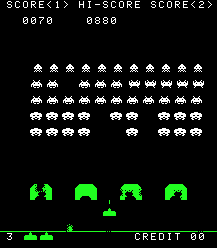
\includegraphics[width=5cm,keepaspectratio]{images/SpaceInvaders-Gameplay}
     }
     \label{fig:figuraInv}
     \fonte{https://en.wikipedia.org/wiki/Space_Invaders}%% Arquivo foi convertido para PNG posteriormente
 \end{figure}
%%%%%%%%%%%%%%%%%%%%%%%%%%%%%%%%%%%%%%%%%%%%%%%%%%%%
% Capítulo 2
%
\chapter{Visão Geral Da Linguagem}

    
%\section{Linguagem Escolhida}
A linguagem escolhida pelo grupo foi Rust. Rust é uma linguagem de programação que tem por objetivo facilitar a execução de âmbitos de programação que costumam ser relegados apenas a códigos de baixo nível, de forma que não seja perdida eficiência tanto de memória quanto de velocidade (Matsakis e Turon 2018) \citet{thebook}. Rust alcança esses objetivos através de sua alta segurança sem que haja necessidade de nenhum agente em tempo de execução, como coletor de lixo, assim como a linguagem C, adicionando  elementos que permitem abstrações, como \textit{Traits} que se assemelham a interfaces da linguagem Java, sem que haja custo em tempo de execução \citet{Traits}.

É possível quebrar parte da segurança de Rust com o uso de blocos de código inseguros, declarados pela palavra-chave \textit{Unsafe}, dentro desses blocos é possível realizar tarefas que não é possível de se realizar em código seguro, como utilizar uma variável estática mutável. Como o foco principal da linguagem é segurança e alta performance, esse relatório estará sempre se referindo a código seguro de Rust, salvo quando seja feita explicita a necessidade de se utilizar código inseguro.

\section{Aspectos Gerais da Linguagem}
A linguagem Rust é uma linguagem compilada fortemente tipada, o que permite que alcance de alta segurança de memória. Em Rust não é possível utilizar uma variável sem iniciá-la, então sempre que é declarada uma variável nova é necessário atribuir um valor a ela antes de utilizá-la. Essas características fazem que Rust seja ótima como uma linguagem de sistemas, por permitir alto controle junto com alta segurança e exatamente por isso já existe sistema operacional escrito nessa linguagem como o sistema redox (\citet{Redox}). 

Os Tipos mais importantes de se compreender para se conhecer melhor a linguagem Rust são os tipos ponteiros, pois a forma como são implementados esses tipos é crucial para entender sobre a segurança de dados e memória da linguagem, assim como a característica de mutabilidade de uma variável. Essas características são em grande parte responsáveis pela segurança de Rust.

\subsection{Tipagem e mutabilidade}

 Em Rust nenhuma variável é mutável a não ser que seja explicitado, exemplo disso é a função \textit{foo1()}  que não é compilada, pois x não é mutável, já a função \textit{foo2()} (funções no trecho de código \ref{lst:mut} \textit{Exemplos de mutabilidade} )não possui erros, assim há proteção da variável a não ser que seja feito explicititada a sua mutabilidade , fazendo com que não seja possível alterar valores de variáveis que não são criadas com essa intenção.

\begin{lstlisting}[frame=single, label={lst:mut}, caption={Exemplos de mutabilidade}]
    fn foo1(){
        let x:usize = 5;
        x=6;
    }
    fn foo2(){
        let mut x:usize = 5;
        x=6;
    }
 \end{lstlisting}

\subsection{Ponteiros Inteligentes}
Em Rust existe o uso de ponteiros, porém diferentemente de linguagens como C e C++, é utilizado ponteiros inteligentes. A diferença dessa forma de utilização de ponteiros, é que o ponteiro possui metadados que visam aumentar a segurança da memória, sendo esses, por exemplo, a quantide de ponteiros a uma região da memória e se apenas um ou mais ponteiros podem acessar essa região. Existem ao todo três tipos diferentes de ponteiros que alocam memóriado no heap, enquanto para alocar memória na pilha basta o uso do operador \textit{\&}. 

Ao usarmos um ponteiro da pilha ou um ponteiro do tipo \textit{Box<T>} haverá sempre apenas uma variável capaz de acessar o seu valor, vide o código \ref{lst:pointers}, onde \textit{foo1()} é compilado sem problemas, mas \textit{foo2()} não é compilado, pois após a atribuição na linha 2 de \textit{foo2()}, a variável b é possuidora do ponteiro, então apenas ela é capaz de acessar suas informações.

 
 
 \begin{lstlisting}[frame=single, label={lst:pointers}, caption={Exemplos de ponteiros}]
    fn foo1(){
        let a = Box::new(5i32);
        let b = a;
        destroy_box(b);
    }
    
    fn foo2(){
        let mut a = Box::new(5i32);
        let b = a;
        destroy_box(b);
        *a = *a+1;
    
    }
 \end{lstlisting}
Existe também ponteiro do tipo \textit{Rc<T>}, em que o mesmo pode possuir mais de uma referência para o mesmo conteúdo e seu metadado executa a contagem de quantas referências existem. Esse ponteiro, entretanto não é seguro para paralelismo quando se mais de uma thread possui uma cópia mutável, pois pode ocorrer corrida por dados. Para que isso não aconteça entre threads a linguagem implementa também o ponteiro \textit{Arc<T>}, esse ponteiro é semelhante ao ponteiro \textit{Rc<T>}, porém utiliza de mutex para fazer acesso ao conteúdo, assim permitindo que seja utilizado em mais de um thread.

\subsubsection{Posse e Empréstimo}
Rust possui duas formas de se utilizar \textit{alias} para os ponteiros. A primeira forma é através de \textit{posse}, essa forma é mostrada no trecho de código \ref{lst:pointers}, onde ao copiarmos a variável \textit{a} para a variável \textit{b}, a primeira deixa de ser acessível, pois agora a segunda é a possuidora do ponteiro. No trecho de código \ref{lst:borrow}, podemos ver um exemplo de \textit{empréstimo}, onde a variável \textit{b} faz o empréstimo do conteúdo de \textit{a} e então sai de escopo. Ao sair de escopo a variável \textit{b} não existe mais e quem lhe fez o \textit{empréstimo}, no caso em questão a variável \textit{a}, volta a possuí-la.


\begin{lstlisting}[frame = single, label ={lst:borrow}, caption = {Exemplo de Empréstimo}]
    fn foo2(){
        let mut a = Box::new(5i32);
        {
            let b = &a;
        }
        *a = *a+1;
    
    }
\end{lstlisting}

\subsubsection{Tempo de vida}
Ponteiros alocados na pilha são desalocados quando acaba seu tempo de vida, então não podem ser acessados ou utilizados por variáveis com tempo de vida diferente. Para permitir que funções retornem ponteiros que não são explicitadamente alocados no monte, como ponteiros \textit{Box<T>}, Rust permite que seja explicitado o tempo de vida de forma separada do escopo. Podemos ver exemplo disso no trecho de código \ref{lst:lifetime}. Como não existe especificação do tempo de vida do retorno, o compilador elide por padrão o tempo de vida do escopo da função, então ao sair do escopo de \textit{foo()}, a memória é desalocada o que resulta no compilador não permitir o retorno, pois estará acessando memória que o compilador prevê já ter sido desalocada.

\begin{lstlisting}[frame =single, label={lst:lifetime},caption={Exemplo de tempo de vida}]
    fn main(){
    
        let x = &mut 3;
        let a = foo(x);
        
    }
    
    fn foo(x:& mut i32) ->& i32{
        *x = *x+2;
        x
    }
\end{lstlisting}

Para resolver esse conflito, devemos especificar o tempo de vida das variáveis da função \textit{foo()}, para assim podermos retornar um ponteiro que não tenha sido desalocado, conforme o trecho de código abaixo \ref{lst:lifetime2}.

\begin{lstlisting}[frame = single, label={lst:lifetime2},caption={Exemplo dois de tempo de vida}]
    fn main(){
        let x = &mut 3;
        let a = foo(x);
        
    }
    
    fn foo<'a>(x:&'a mut i32) ->&'a i32{
        *x = *x+2;
        x
    }
\end{lstlisting}

\section{Paradigma Funcional}
Ao trabalhar com Rust focando-se no paradigma funcional, é visto que a linguagem não foi construída com esse paradigma como foco principal, apesar de possuir diversas características para ser considerada uma linguagem funcional. Rust é, na verdade, uma linguagem multiparadigma, que entre seus paradigmas está o paradigma funcional, possuindo tipos imutáveis, funções anônimas e outros recursos recorrentes do paradigma funcional.
%apesar de possuir suporte a diversos itens desse paradigma. O principal motivo para isso é devido a forma como são utilizados parâmetros de funções, pois, para diversos tipos a passagem de parâmetro é feita apenas por referência, podendo, assim, resultar em efeitos colaterais nas funções. Com o intuito de contornar isso, não gerar efeito colateral e o ponteiro não ser movido, é criado um cópia do argumento que é utilizado apenas para a chamada da função, assim, mesmo que gere efeito colateral, ele não será propagado, consequentemente temos a percepção de que o argumento está sendo passado por valor.


\section{Paradigma Orientado a Objetos}
 Rust não possui suporte ao paradigma orientado a objetos, dentre os motivos estão, pois não possui diversas características naturais a esse paradigma. Dentre essas características está o fato de que em Rust não é possível se definir classes, conceito essencial para que se utilize diversos recursos desse paradigma. Apesar desses fatores, Rust possui estruturas capazes de possuir métodos e também interfaces, aqui chamadas de \textit{Traits}, elementos que aproximam Rust desse paradigma e que permitem contornar a falta de suporte ao paradigma e podermos recriar características como classes, através de módulos, para encapsulamento, \textit{structs}, para definição de atributos, e interfaces, para a definição de métodos que devem ser herdados.

%%%%%%%%%%%%%%%%%%%%%%%%%%%%%%%%%%%%%%%%%%%%%%%%%%%%%%%%%%%%%%%%%%%%%%%%%%%%%%%%%%%%%
% Capítulo 3
%
\chapter{Elementos Funcionais}

\section{Funções puras e elementos imutáveis}
Funções puras são funções que não causam efeito colateral, ou seja, não há alterações fora de seu próprio escopo. Em Rust alguns tipos resultam em mudança de posse ou em empréstimo ao serem utilizados como parâmetros. No caso de mudança de posse não resulta em efeito colateral, porém a variável que usamos como parâmetro é perdida, já no caso de empréstimo não perdemos a variável, porém o empréstimo é semelhante a passagem por referência, então pode resultar em efeitos colaterais. Existem duas formas para resolvermos isso em Rust.

A primeira forma é a utilização de tipos imutáveis nos parâmetros, ou seja, a não ser que seja explicitado a mutabilidade do parâmetro, não é possível fazer alterações nessa variável, mesmo que seja passada por referência.

A segunda forma é a utilização de clones. Diversos tipos em Rust possuem uma função clone que cria uma cópia profunda da variável. Ao utilizarmos essa cópia como argumento para a chamada de função, por mais que seja passada por referência não gerará efeito colateral e, caso seja feita a mudança de posse, não perderemos a referência a variável original.

Exemplos para esses dois casos, encontramos na função \textit{move\_right} que recebe 2 variáveis como parâmetros, sendo uma delas mutavel e outra não, mas ao fazer a chamada da função é utilizado o método clone, como foi explicitado anteriormente.


\begin{lstlisting}[frame = single]
    let line_temp  = move_right(chars_p.next(),
     chars_p.clone(),'-');

\end{lstlisting}
\begin{lstlisting}[frame=single, label ={lst:purefn}]
    fn move_right
        (indiv: Option<char>,mut  _line:std::str::Chars<'_>,
            new_char:char)-> String{
        let mut buf = String::with_capacity(5);
        match indiv{
            Some(x)=>{
                buf.push(new_char);
                buf.push(x);
                return move_rest_right
                    (_line.next().clone(),
                    _line.clone(), buf.clone());
                
            } ,
            None=> buf = String::new(),
        }
        buf
    }
\end{lstlisting}


    

 
 




\section{Funções anônimas}
Rust possui suporte para o uso de funções anônimas através de closures. Foi utilizado função anônima para a chamada da função \textit{move\_one\_char}, onde foi utilizada uma closure como argumento para a chamada da função

\begin{lstlisting}[frame=single, label = {lst:anon}]
    let new_line = move_one_char(screen[0].clone(),
     |y:char|if y == ALIEN{BLANK_SPACE}else{SHOT_OBJ});


\end{lstlisting}

\section{Currying}
    O foco de currying é transformar uma função que possua diversos parâmetros em uma função que receba apenas um. A forma como foi utilizada foi através de funções de alta ordem e função anônima, conforme o trecho código abaixo, a função \textit{victory\_condition} recebe uma variável do tipo \textit{String} e retorna uma função que recebe uma variável do tipo \textit{char}.
    
    
\begin{lstlisting}[frame=single, label = {lst:curr}]
    fn victory_condition(vec:String)-> impl Fn(char)->bool{
       move |x| vec.contains(x)
    }
\end{lstlisting}
Podemos ver o uso dessa função no seguinte trecho, onde primeiro par de parênteses analisa o paraâmetro \textit{x} e o segundo é a chamada da função de retorno, responsável por analisar o segundo parâmetro.

\begin{lstlisting}[frame = single]
    let ans:Vec<bool> =alien_space.into_iter().map(|x|
    victory_condition(x)(ALIEN)).collect();

\end{lstlisting}

\section{Pattern matching}
Pattern matching é uma ferramenta para identificação de padrões simples em estruturas de dados, foi utilizado o operador \textit{match}, para identificar padrões dentro de \textit{enums}, como no trecho de código a seguir, onde \textit{indiv} é um enum que identifica se possui existe valor ou não dentro de uma estrutura de dados, como um vetor.

\begin{lstlisting}[frame = single]
    match indiv{
        Some(x)=>{
            if  (x == ALIEN) || (x == PLAYER){
               return String::new(); 
            }
            return move_rest_left(_line.next().clone(),
             _line.clone(), buf.clone(), new_char);
            
        } ,
        None=> return String::new(),
    }
    
\end{lstlisting}

\section{Funções de Ordem Superior}
 São consideradas funções de ordem superior, funções que possuem como parâmetro uma outra função ou retornam uma função. Exemplo de forma como foi utilizado esse conceito no projeto é a função\textit{move\_one\_char}.
 
 \begin{lstlisting}[frame=single, label ={lst:ordemsup},caption={\textit{função move\_one\_char}}]
    fn move_one_char<F>(mut s:String, resolve:F)-> String
     where F: Fn(char)->char{
 
\end{lstlisting}
Essa função recebe uma \textit{String}, que seu primeiro elemento irá mover apenas um caracter para o lado, e uma função que resolve o que deve acontecer ao realizar esse movimento. E a função \textit{resolve} é chamada no seguinte trecho.
\begin{lstlisting} [ frame = single]
    let first =  s.remove(length);
    let second = s.remove(length-1);
    let result = resolve(second);
 \end{lstlisting}
 
 
 
 \section{Funções de ordem maior fornecidas pela linguagem}
 Rust possui diversas funções de ordem maior, como a função \textit{spawn}, que cria uma nova thread que executa a função passada como argumento e afunção \textit{map} que aplica uma função a um elemento iteravel, ambas funções foram utilizadas no projeto conforme os exemplos.
 
 \begin{lstlisting}[frame=single]
    let mut handle = Future::spawn(move|| read_input());
 \end{lstlisting}
 \begin{lstlisting}[frame=single]
let ans:Vec<bool> =alien_space.into_iter().
    map(|x| return victory_condition(x)(ALIEN)).collect();
 \end{lstlisting}

 \section{Funções como Elementos de Primeira Ordem}
 Funções são tratados como elementos de primeira ordem quando podem ser utilizadas como parâmetro de outras funções, exemplo disso já mostrado no trecho de código \ref{lst:ordemsup} \textit{move\_oner\_char}.
 
 
\section{Recursão}
Recursão foi utilizado em diversas funções, entre elas está a função \textit{move\_right} \ref{lst:purefn} citada anteriormente. Essa função utiliza da recursão para percorrer por toda uma string.

 
 \chapter{Recursos De Orientação a Objetos}

 
 \section{Classes}
 Como comentado anteriormente Rust não possui suporte a classes, então para a reprodução de uma estrutura de classes foram utilizadas \textit{Structs}, para o armazenamento dos atributos e implementação dos métodos. Para a declaração de métodos ue devem ser herdados por classes filhos foram utilizadas \textit{Traits}, pois elas permitem herança de outra \textit{Trait}. Para fazer o encapsulamento dos atributos foram utilizados \textit{Módulos}, pois em Rust não existe encapsulamento dentro de um arquivo e o uso de módulos nos auxilia na separação do código em diferentes arquivos.
 \begin{lstlisting}[frame = single]
    pub struct Base{
        position: (i8,i8),
        img:char,
    }
    pub trait BaseT{
        fn get_img(&self)->char;
        fn get_position(&self)->(i8,i8);
        fn set_pos(& mut self,npos:(i8,i8));
    }
    impl BaseT for Base{
        fn get_position(&self)->(i8,i8){
            return self.position;
        }
    
        fn get_img(&self)->char{
            return self.img;
        }
        fn set_pos(& mut self,npos:(i8,i8)){
            self.position = npos;
        }
    }
    
 \end{lstlisting}
 
 
 
 \section{Encapsulamento e proteção de atributos}
  A linguagem Rust, possui apenas a possibilidade de atributos privados ou públicos, pois como não existe herança na linguagem, o conceito de atributo protegido não seria condizente. Para se recriar variáveis protegidas se utilizou da forma de estrutura de arquivos e módulos de Rust. Com o uso de módulos podemos declarar classes em módulos separados, para manter a privacidade dos atributos, e classes filhas no mesmo módulo dentro do mesmo arquivo, assim todos os atributos privados do arquivo são acessíveis a todas as estruturas ali implementadas. No trecho de código abaixo vemos a classe \textit{Player} acessando uma variável declarada privada de \textit{Base}, fazendo com que a mesma seja protegida. Já as classes declaradas fora desse módulo não terão acesso.
  
  \begin{lstlisting}[frame = single]
    impl BaseT for Player{
        fn get_img(&self)->char{
            self.my_base.img
        }
  \end{lstlisting}
  No código abaixo
  
 %%%Adicionar Código
 
\section{Construtores}
 Em Rust existem construtores para as \textit{structs} que já realizam a alocação de memória necessária, então foram criados apenas construtores para as classes criadas de forma a fazer com que todas as variáveis possuam valores válidos. Para esses construtores das classes foram utilizados métodos com a palavra \textit{new} no nome, como não é possível se ter mais de uma função com o mesmo nome, foram utilizados nomes diferentes, mas todos possuindo a palavra \textit{new}. 
 
 \begin{lstlisting}[frame =single]
    impl GameObjectT<Base> for Base{
        fn new( _position:(i8,i8))->Base{
            Base{
                position : _position,
                img: GameImages::None.value(),
            }                        
        }
        fn new_wbase(_base:Base) ->Base{
            _base
        }
    }
 \end{lstlisting}
 
 \section{Destrutores}
 Em rust existe uma \textit{Trait}, chamada \textit{Drop}, que implementa destrutores de forma genérica para todos os tipos básicos da linguagem. Como dito no capítulo 15 do livro \citet{thebook} o compilador reconhece quando uma variável sai de escopo e realiza a chamada do destrutor nesse momento, para variáveis alocadas na pilha, as mesmas são desalocadas quando a função acaba e o frame pointer é movido. Dessa forma então não existe a necessidade de implementar destrutores ou fazer chamadas a destrutores.
 
 Como mostrado no site \citet{Drop101}, podemos implementar destrutores para tipos nomeados, porém esses destrutores devem ser utilizados apenas quando há necessidade de fazer algo especial além de desalocar a memória, como dito pelo usúario \textit{masklinn} no post \citet{Dropredd}. Com isso temos então que podemos criar destrutores customizados, porém não existe a necessidade, pois a liberação da memória já é realizada sem necessidade de acréscimo de código
 
 
 \section{Espaços de nome diferenciados}
 Módulos em Rust permitem que a separação e organização do código e também a visibilidade de atributos. Podem  podem ser construídos varios módulos dentro de um mesmo arquivo, porém nesse caso não existiria proteção de atributos dentro do mesmo arquivo. Então é necessário que sejam criados módulos para cada super classe e todas as classes filhas sejam no mesmo arquivo para que se possa utilizar de atributos protegidos. Outra utilização de módulo foi para a definição de \textit{Enums} de erros, assim permitindo que uma função retorne de forma explicita que ocorreu um erro em sua execução.
 
 \begin{lstlisting}[frame= single]
    pub mod game_object;
    pub mod game_screen;
    pub mod errors{
        use super::game_object::GameObjectClass;
        #[derive(Copy,Clone)]
        pub enum ScreenLimit{
            Err,
            Ok((i8,i8)),
        }
        pub enum CollisionErr{
            Err,
            Ok(GameObjectClass),
            Die,
        }
    }
 \end{lstlisting}
 
 \section{Mecanismos de Herança}
 A linguagem possui suporte a herança de \textit{Traits}, então foi utilizado disso para que, com isso, possamos garantir que uma classe filha implemente todos os métodos da classe pai, porém isso não garante que o filho herde os atributos da classe pai. Para que haja herança de atributos foi utilizado que o filho possua um atributo da classe pai, assim temos não só a herança dos atributos da classe pai, mas como também acesso às implementações dos métodos pela classe pai. Foi utilizado implementações de struct para métodos que não são públicos, assim esses métodos não são herdados de forma a poderem ser reimplementadas.
 
No projeto foi utilizado herença para a criação dos objetos de jogo. Foi criada uma classe básica, chamada \textit{base}, essa classe será a classe pai de todos os objetos de jogo e possui os atributos que são compartilhados por todas. Essa classe possui uma \textit{Trait} atrelada a si que é \textit{BaseT}.

\begin{lstlisting}[frame = single]
    pub struct Base{
        position: (i8,i8),
        img:char,
    }
\end{lstlisting}

\begin{lstlisting}[frame = single]
    pub trait BaseT{
        fn get_img(&self)->char;
        fn get_position(&self)->(i8,i8);
        fn set_pos(& mut self,npos:(i8,i8));
    }
\end{lstlisting}
 Uma classe filho é delcarada da seguinte forma para possuirmos a herança de \textit{Base}. Quando \textit{PlayerT} for ser implementada para a classe \textit{Player}, o compilador irá retornar erro de compilação caso todos os métodos de \textit{BaseT} não sejam implementados também.
 
 \begin{lstlisting}[frame = single]
    pub struct Player{
        my_base:Base,
        lifes:i32,
    }
 \end{lstlisting}
 
 \begin{lstlisting}[frame = single]
    pub trait PlayerT: GameObjectT<Player> + BaseT{
        fn walk(& mut self,dir:bool,right_limit:i8)->
        errors::ScreenLimit;
        
        fn shoot(& mut self)->Shot;
        fn die(&mut self)->i32;
        fn get_lifes(&self)->i32;
        fn gain_life(&mut self)->i32;
    }
 \end{lstlisting}
 
 \section{Polimorfismo paramétrico}
%fn <T>
 Rust fornece suporte a polimorfismo paramétrico e também suporte a restrições desse tipo, tanto para funções quanto para \textbf{Traits}. Então foi utilizado polimorfismo paramétrico com restrições para a implementação de um contrutor genérico para toda classe que implemente a \textit{Trait GameObjectT} para o seu próprio tipo.
 
 
 \begin{lstlisting}[frame = single]
     fn new_img<A:GameObjectT<A>>(_img:char,
        _position:(i8,i8))->A{
        let nb = Base{
            position : _position,
            img: _img,
        };
        let na:A = A::new_wbase(nb);
        return na;
    }
 \end{lstlisting}
 
 \section{Polimorfismo por sobrecarga}
 Pode-se ver um exemplo de polimorfismo por sobrecarga na classe \textit{Player}, que herda o método \textit{set\_pos} da classe \textit{Base}, mas não utiliza a implementação da classe pai, pois um objeto \textit{Player} não pode ter sua posição alterada  sem utilizar o método \textit{walk}, então em sua implementaçã não possui nenhuma instrução.
 
 \begin{lstlisting}[frame=single]
    //Classe filho
    fn set_pos(& mut self,npos:(i8,i8)){
        
    }
    //Classe mãe
    fn set_pos(& mut self,npos:(i8,i8)){
        self.position = npos;
    }
 \end{lstlisting}
 
 \section{Delegates}
Delegate é um elemento que permite a avaliação de um objeto no contexto de um segundo objeto. Para exemplificar esse conceito foi utilizado um delegate para avaliar as colisões entre objetos, assim a forma o resultado das colisões é mais fácil de alterar sem necessitar alterar as classes criadas para o projeto.
\begin{lstlisting}[frame= single]
    fn move_world(&mut self,delegate_collision:
    fn(GameObjectClass,GameObjectClass,&mut i32)->
    errors::CollisionErr);
\end{lstlisting}
Quando feita a chamada da função é passada uma função declarada fora de qualquer uma das classes, mas quando é executada ela será executada no escopo da classe \textit{GameWorld}.
\begin{lstlisting}[frame = single]
    gw.move_world(collision);

\end{lstlisting}
 
 \begin{lstlisting} [frame = single]
    let mv_res =a.move_alien
     (self.speed,limits.0,limits.1,self.cur_dir);
    match mv_res{
        errors::ScreenLimit::Err=>{
            return errors::ScreenLimit::Err;        
        },
        errors::ScreenLimit::Ok(o)=>{
            let al_n_pos = a.get_position();
            let old = new_screen
             [al_n_pos.0 as usize][al_n_pos.1 as usize];
            let res = delegate_collision( GameObjectClass::
            Alien(AliensClass::SupAlien(a)),old,
            &mut self.points);
 \end{lstlisting}
 
 \chapter{Recursos de processamento paralelo}   
 Rust possui em sua biblioteca padrão funções para criação e gerenciamento de threads, entretanto foi utilizada a biblioteca \textit{eventual}, pois ela nos permite receber o retorno de uma thread sem que a necessidade de parar a execução para esperar. a função \ref{lst:readinput}\textit{read\_input} espera a entrada do usuário sem esperar pela tecla enter e retorna essa entrada.
 
 \begin{lstlisting}[frame=single, label={lst:readinput},caption={Função read\_input}]
    fn read_input() -> char{
        let stdin = 0; 
        let termios = Termios::from_fd(stdin).unwrap();
        let mut new_termios = termios.clone();  
        new_termios.c_lflag &= !(ICANON | ECHO); /
        tcsetattr(stdin, TCSANOW, &mut new_termios).unwrap();
        let stdout = io::stdout();
        let mut reader = io::stdin();
        let mut buffer = [0;1];
        
        stdout.lock().flush().unwrap();
        reader.read_exact(&mut buffer).unwrap();
        let a: char= char::from(buffer[0]);
        //println!("You have hit: {}", a);
        tcsetattr(stdin, TCSANOW, & termios).unwrap();  
        return a;
    }
 \end{lstlisting}
 
 A criação da thread está declarada no trecho de código \ref{lst:parum} dentro da função \textit{main}. Já no trecho de código \ref{lst:pardois} é feito um teste para verificar se a thread que está sendo controla pela variável \textit{handle} já concluiu a execução, caso sim é criada a variável \textit{data} para receber o retorno da função, criada uma nova thread para executar novamente a função \textit{read_input} e então dentro do bloco de código do operador \textit{match} é feito a análise da entrada do usuário. 
 
 \begin{lstlisting}[frame = single, label = {lst:parum},caption={Criação da thread}]
     let mut handle = Future::spawn(move|| read_input());

 \end{lstlisting}
 \begin{lstlisting}[frame=single,label={lst:pardois},caption={Retorno da thread}]
    if handle.is_ready(){
        let data =handle.expect().unwrap();
        handle = Future::spawn(move|| read_input());
        match data{
 \end{lstlisting}
 
 \section{Gerência de Regiões Críticas}
Como falado anteriormente, o sistema de tipos de Rust já realiza a gerência de regiões críticas, entã não existe a necessidade de realizarmos isso. Tendo isso em vista, na solução funcional foi utilizida uma região insegura de código da memória, para podermos alterar uma variável global. Como esse trecho não acontece em mais de uma thread, não houve necessidade gerenciar esse acesso.

\begin{lstlisting}[frame=single]
    unsafe{
        alien_screen =move_aliens(alien_screen.clone(),
         MOVEMENT_DIRECTION);
   }
\end{lstlisting}
 
%%%%%%%%%%%%%%%%%%%%%%%%%%%%%%%%%%%%%%%%%%%%%%%%%%%%%%%%%%%%%%%%%%%%%%%%%%%%%%%%%%%%%
% Conclusões
%
\chapter{CONCLUSÃO Final}
Para o desenvolvimento funcional, Rust se mostrou uma ótima linguagem, pois possui suporte a quase todas as características funcionais. Com isso foi possível resolver o problema de forma satisfatória replicando elementos básicos do jogo, como movimentar o personagem, atirar e movimentar os alienígenas. 


No âmbito de orientação a objetos, Rust houve necessidade de criar diversos contornos para poder-se replicar características importantes desse paradigma, já que a linguagem não possui suporte a poucas das caracterísiticas desse paradigma. Mesmo com esse empecilho, o desenvolvimento em orientação a objetos permitiu que se utilizasse os pontos fortes de abstrações que se possui em Rust, que são as \textit{Traits} e os \textit{Smart Pointers}, podendo assim haver mais reaproveitamento de código.

Abaixo podemos ver a tabela de avaliação geral da linguagem, nela podemos ver que que Rust é uma linguagem focada em segurança,  e os pontos relacionados  ela realiza com sucesso, como restrição de aliasing, entretanto a mesma possui baixa ortogonalidade, pois como é fortemente tipada e não possui coerções implicitas ou diversidade de operadores entre tipos diferentes, acabam sendo poucos os tipos diferentes que podem ser operados entre si. A portabilidade é baixa, pois como é compilada é necessário que haja compiladores para as diferentes arquiteturas e sistemas operacionais, além do fato de existirem bibliotecas específicas para sistema operacional. Vemos também que em Rust não existem exceções, porém a linguagem utiliza de tipos \textit{Enums} para fazer retornos de erro e possui uma funç

, chamada \textit{panic}%ão parebobinar a pilha em caso de não poder ser recuperado o estado de execução.ra %%%%
Com essas informações vemos que Rust é uma linguagem muito forte nos pontos onde seus criadores se propuseram a realizar, como segurança de memória, porém em diversos pontos ligados a produtividade e redigibilidade ela falha em alcançar qualidade semelhante a que alcança nos pontos ligados a segurança. Temos então que Rust é uma linguagem de sistema capaz de concorrer com linguagens já estabelicidas, entretanto ela falha em quesitos importantes para se ter alta produtividade de maneira fácil, como simplicidade ou ortogonalidade.



\begin{figure}[htb]
     \centering
     \caption{Tabela de avaliação da linguagem}
     \fbox{
         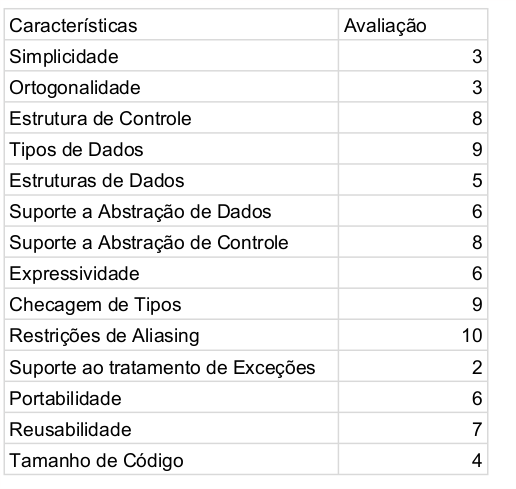
\includegraphics[width=10cm]{images/lang table.png}
     }
     \label{fig:figuraInv}
 \end{figure}

%%%%%%%%%%%%%%%%%%%%%%%%%%%%%%%%%%%%%%%%%%%%%%%%%%%%%%%%%%%%%%%%%%%%%%%%%%%%%%%%%%%
% Referências 
%%%%%%%%%%%%%%%%%%%%%%%%%%%%%%%%%%%%%%%%%%%%%%%%%%%%%%%%%%%%%%%%%%%%%%%%%%%%%%%%%%%
%

%\bibliographystyle{abnt}

\bibliographystyle{abntex2-alf}

\bibliography{biblio} % arquivo que contém as referências (no formato bib). Colocar as suas lá (se tiver dúvida sobre como adicionar novas referências, usar o software JabRef ou Medley)





\end{document}
